% !TeX spellcheck = pt_PT
\documentclass[12pt,a4paper]{article}
\usepackage[portuguese]{babel}
\usepackage[utf8]{inputenc} 
\usepackage{natbib}
\usepackage{graphicx}
\usepackage{listings}
\author{André Cirne e José Sousa}
\title{Aprendizagem máquina e o ID3}
\begin{document}
	
\begin{titlepage}
	\centering
	{\scshape\LARGE Faculdade de Ciências \par}
	\vspace{1cm}
	{\scshape\Large Inteligência Artificial\par}
	\vspace{1.5cm}
	{\huge\bfseries Trabalho 4\par}
	\vspace{2cm}
	{\Large\itshape André Cirne e José Sousa\par}
	\vfill
	
	{\large \today\par}
\end{titlepage}

\tableofcontents

\section{Introdução}
Uma árvore de decisão é a representação de uma função que através de uma prévia a avaliação de um determinado conjunto de dados, consegue retornar uma decisão para uma nova situação\cite{stuart2016artificial}. A utilização de uma árvore de decisão é o método de representação de dados que nos permite ser mais simples e obter uma maior taxa de sucesso quando utilizados em conjunção com algoritmos de indução em árvores de decisão.

Numa árvore de decisão cada nó representa um teste ao conjunto de dados que se pretende avaliar e em cada um dos seus ramos encontra-se identificado os possíveis valores que este pode tomar. Estes testes e os seus ramos vão conduzindo o algoritmo até a um nó folha aonde se encontra o valor a ser retornado pela função, que será a sua decisão.

\section{Algoritmos de indução de árvores de decisão}
As árvores de decisão são apenas uma estrutura de dados, logo sem algoritmos capazes de construir estes modelos de previsão de forma eficiente, elas não servem para nada.

Os algoritmos de indução de árvores de decisão são algoritmos que dado um conjunto de dados exemplo consegue representar de forma genérica as relações existentes entre estes e um determinado acontecimento que estamos a considerar como resultado e partindo destas relações constroem de forma automática a árvore de decisão.\cite{rokach2005top} Estes algoritmos por norma aplicam princípios \textit{greedy}, utilizando métricas para efetuar a escolha de nós ao longo da construção da árvore.

\subsection{Métricas}

\subsubsection{Ganho de informação}
O ganho de informação é baseado no conceito de entropia. A entropia é a media de incerteza que há num sistema. Usando o conceito de entropia podemos calcular a probabilidade de ocorrência de um determinado evento em cada conjunto de resultados.
Dado um conjunto S, com instâncias pertencentes à classe i, com probabilidade  $\phi$, temos:

\begin{equation}
	Entropia = \sum_{i} \phi\log\phi
\end{equation}

\subsubsection{Impuridade de Gini}
A impuridade Gini é uma métrica que mede a divergência entre a distribuição probabilística  dos valores que um atributo toma.
Dado um conjunto S,  com instâncias pertencentes à classe j, com probabilidade  $\phi$, temos\cite{teknomo2017dec}:

\begin{equation}
	Impuridade_de_Gini = 1 - \sum_{j} \phi^{2}
\end{equation}

\subsection{ID3}
O algoritmo ID3 (inductive decision tree) é um dos algoritmos mais utilizados para a construção de árvores de decisão. Este algoritmo utiliza princípios \textit{greedy}, escolhendo assim em cada nó da árvore aquele que acha que lhe permitirá alcançar uma árvore mais compacta. Para esta escolha do melhor atributo utiliza como métrica o ganho de informação. 
O ID3 segue os seguintes passos:
\begin{enumerate}
	\item 	Começar com todos os exemplos de treino;
	\item	Escolher o teste (atributo) que melhor divide os exemplos, ou seja agrupar exemplos da mesma classe ou exemplos semelhantes;
	\item	Para o atributo escolhido, criar um nó filho para cada valor possível do atributo;
	\item	Transportar os exemplos para cada filho tendo em conta o valor do filho;
	\item	Repetir o procedimento para cada filho não "puro". Um filho é puro quando cada atributo X tem o mesmo valor em todos os exemplos. 
\end{enumerate}

\subsection{CART}
CART que significa "Classification and Regression Trees" é um algoritmo caracterizado pela construção de árvores de decisão binárias.\cite{rokach2005top} É um algoritmo que não só constrói árvores de classificação mas sim também árvores de regressão, dependendo se a variável em questão é categórica ou numérica. Como métrica para o ganho utiliza a impuridade de gini.
O algoritmo segue as seguinte regras para a construção de árvores de decisão:
\begin{enumerate}
	\item Os valores das variáveis são escolhidos de forma a que divisão seja a melhor a possível.
	\item Logo que a divisão se aplique a este processo é aplicado aos seus filhos.
	\item Esta divisão acaba quando o CART deteta que já não existe nenhum ganho ao fazer a divisão ou no caso da existência de outra regra que ja foi previamente identificada.  
\end{enumerate}

\subsection{C4.5}
O algoritmo C4.5 é um melhoramento do algoritmo ID3, isto devido ao fato de se encontrar preparado para trabalhar com valores contínuos e discretos. 
Outros dos melhoramentos é a possibilidade de existência de atributos não avaliados num determinado grupo de dados de exemplo. Quando num determinado exemplo existe um atributo sem valor este não entra para o calculo da métrica.
Além disto tudo o melhoramento mais interessante deste algoritmo é que quando este acaba a construção de uma árvore de decisão tenta pudar ramos da árvore que não sejam necessários e substitui-los por nós folha.
Trabalhar com atributos que possuem valores indisponíveis na construção de uma árvore da decisão, pode ser considerado um problema. 
Fora as diferenças anteriormente referidas este algoritmo é equivalente e graças a estes melhoramentos o C4.5 consegue obter árvores mais simples quando comparadas com o ID3. 

\section{Implementação}
Neste trabalho utilizamos Python 3, devido a ser uma linguagem multi-paradigma e levando assim a uma passagem mais rápida da parte do planeamento para implementação.
A forma como era necessário responder ao problema obrigava-nos a que por um lado conseguíssemos representar e construir de forma organizada uma árvore de decisão capaz não só de armazenar dados brutos mas por exemplo no caso de dados numéricos conseguir agrupá-los de forma a que a árvore se torne mais legível, sem comprometer a sua fiabilidade.  
\subsection{Estrutura de dados}

\subsubsection{Dicionários e listas}
Ao longo da implementação foram utilizadas listas devido à sua modularidade, suportando qualquer tipo de valor. E dicionários devido ao seu poder de organização já que podemos associar duas estruturas de dados e utilizar uma delas como chave.

\subsubsection{Leaf}
Estrutura com o objetivo de representar os nós folhas na árvore de decisão. Aqui estará armazenado a resposta ao nó pai, a classe e o contador dos casos que se encontram identificados com esta folha.
%\begin{figure}
%	\centering
%	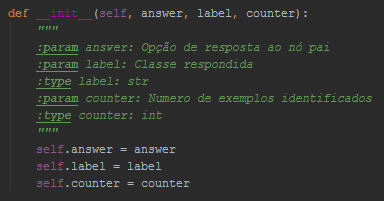
\includegraphics[]{img/leaf.png}
%	\caption{Inicialização da classe leaf.}
%\end{figure}
\subsubsection{Jump}
Esta estrutura é o elo de ligação entre dois nós da árvore  de decisão, a estrutura Jump é composta por um campo answer com a resposta ao nó pai , um contador com o número de nós que se identificaram com aquele caso e um apontador para outro nó da árvore.
%\begin{figure}
%	\centering
%	\includegraphics[]{img/jump.png}
%	\caption{Inicialização da classe jump.}
%\end{figure}
\subsubsection{Node\_root}
Estrutura que representa cada nó da árvore as suas componentes principais é o atributo e uma lista com todos os deus ramos.
%\begin{figure}
%	\centering
%	\includegraphics[]{img/node.png}
%	\caption{Inicialização da classe Node\_root.}
%\end{figure}

\subsection{Intervalo}
A estrutura intervalo, é aquela que nos permite que consigamos representar intervalos numéricos na árvore de decisão. Da forma como ela foi implementada permite a ordenação de intervalos de forma automática e quando a estrutura intervalo é comprada com um valor numérico se esse se encontrar nos seus limites identifica-o como seu.

\subsection{Organização do código e implementação}
A organização deste código foi feita através da criação de um classe chamada decision tree, ao inicializar esta classe é construida a árvore de decisão utilizando o algoritmo ID3. Neste processo de construção também é efetuado a transformação de valores numéricos em intervalos numéricos. 

No cálculo do ID3 utilizámos como heurística a entropia para a decisão de quem é que vai ser o atributo a ser escolhido para um nó da árvore. É importante referir que no caso de a uma dada altura na construção da árvore existir um ramo que não tenha qualquer exemplo com o qual possamos atribuir um valor, a este é atribuído o valor mais comum da árvore. A implementação tenta trabalhar com base em recursão pelas várias classes.

Além da implementação em si do algoritmo também foi necessário implementar um parser para a leitura de CSV, sempre que queremos testar um determinado conjunto de dados ou como conjunto de dados exemplo para a construção da árvore de decisão, esta tarefa foi nos facilitada pela  linguagem de programação que escolhemos já que esta possui módulos próprios para leitura de CSV's.  

\section{Resultados}

\subsection{restaurant.csv}
\begin{lstlisting}
<Pat>
	Some: Yes (4)
	None: No (2)
	Full:
		<Hun>
			No: No (2)
			Yes:
				<Type>
					Italian: No (1)
					Burger: Yes (1)
					Thai:
						<Fri>
							No: No (1)
							Yes: Yes (1)
					French: Yes (0)
\end{lstlisting}

\subsection{weather.csv}
\begin{lstlisting}
<Weather>
	overcast: yes (4)
	sunny:
		<Humidity>
			65.0 <= x < 75.0: yes (2)
			75.0 <= x < 96.1: no (3)
	rainy:
		<Humidity>
			65.0 <= x < 75.0: no (1)
			75.0 <= x < 86.0: yes (2)
			86.0 <= x < 95.0: no (1)
			95.0 <= x < 96.1: yes (1)
\end{lstlisting}

\subsection{iris.csv}
\begin{lstlisting}
<petallength>
	1.0 <= x < 3.0: Iris-setosa (50)
	3.0 <= x < 4.5: Iris-versicolor (29)
	4.5 <= x < 4.7:
		<sepallength>
			4.3 <= x < 4.9: Iris-setosa (0)
			4.9 <= x < 5.0: Iris-virginica (1)
			5.0 <= x < 5.4: Iris-setosa (0)
			5.4 <= x < 5.5: Iris-versicolor (1)
			5.5 <= x < 5.6: Iris-setosa (0)
			5.6 <= x < 5.8: Iris-versicolor (2)
			5.8 <= x < 6.0: Iris-setosa (0)
			6.0 <= x < 6.3: Iris-versicolor (4)
			6.3 <= x < 6.4: Iris-setosa (0)
			6.4 <= x < 6.7: Iris-versicolor (3)
			6.7 <= x < 8.0: Iris-setosa (0)
	4.7 <= x < 4.8: Iris-versicolor (5)
	4.8 <= x < 4.9:
		<sepallength>
			4.3 <= x < 5.9: Iris-setosa (0)
			5.9 <= x < 6.0: Iris-versicolor (1)
			6.0 <= x < 6.1: Iris-virginica (1)
			6.1 <= x < 6.2: Iris-setosa (0)
			6.2 <= x < 6.3: Iris-virginica (1)
			6.3 <= x < 6.8: Iris-setosa (0)
			6.8 <= x < 6.9: Iris-versicolor (1)
			6.9 <= x < 8.0: Iris-setosa (0)
	4.9 <= x < 5.0:
		<sepalwidth>
			2.0 <= x < 2.5: Iris-setosa (0)
			2.5 <= x < 2.6: Iris-versicolor (1)
			2.6 <= x < 2.7: Iris-setosa (0)
			2.7 <= x < 2.9: Iris-virginica (2)
			2.9 <= x < 3.0: Iris-setosa (0)
			3.0 <= x < 3.1: Iris-virginica (1)
			3.1 <= x < 3.2: Iris-versicolor (1)
			3.2 <= x < 4.5: Iris-setosa (0)
	5.0 <= x < 5.1:
		<sepallength>
			4.3 <= x < 5.7: Iris-setosa (0)
			5.7 <= x < 5.8: Iris-virginica (1)
			5.8 <= x < 6.0: Iris-setosa (0)
			6.0 <= x < 6.1: Iris-virginica (1)
			6.1 <= x < 6.3: Iris-setosa (0)
			6.3 <= x < 6.4: Iris-virginica (1)
			6.4 <= x < 6.7: Iris-setosa (0)
			6.7 <= x < 6.8: Iris-versicolor (1)
			6.8 <= x < 8.0: Iris-setosa (0)
	5.1 <= x < 7.0:
		<sepallength>
			4.3 <= x < 5.8: Iris-setosa (0)
			5.8 <= x < 6.0: Iris-virginica (4)
			6.0 <= x < 6.1: Iris-versicolor (1)
			6.1 <= x < 6.6: Iris-virginica (15)
			6.6 <= x < 6.7: Iris-setosa (0)
			6.7 <= x < 8.0: Iris-virginica (22)
\end{lstlisting}

\section{Conclusões}
A implementação do algoritmo ID3 em parte aproximou-se do C4.5 já que tivemos de efetuar um dos vários melhoramentos que este possui em relação ao ID3, que foi a preparação para a receção de argumentos numéricos, fazendo o processamentos destes em intervalos e assim tornar a árvore de decisão menos complexa.

Durante a fase de já testes do programa chegámos à conclusão que não era necessário ter utilizado a estrutura jump e a estrutura leaf de forma tão complicada já que nos tinha bastado implementar um dicionário onde a \textit{answer} seria a key de pesquisa no dicionário que ai estaria associada a uma leaf ou a um Node\_root.
\bibliographystyle{plain}
\bibliography{bibliografia} 

\end{document}

